\chapter{Demostración y análisis del sistema}

En este capítulo se recorre la aplicación desde el punto de vista del usuario final y se analizan las visualizaciones principales, explicando qué muestra cada una y cómo interpretarla.

\section{Páginas implementadas}

A continuación se describen las vistas principales de la aplicación y su propósito.

\subsection{Página principal}
La página principal o ``home'' se ha buscado que sea muy sencilla, sólo se muestra el nombre dado a la plataforma, MIMIC-IV Analytics, junto a un pequeño subtítulo. 
\begin{figure}[H]
  \centering
  \fbox{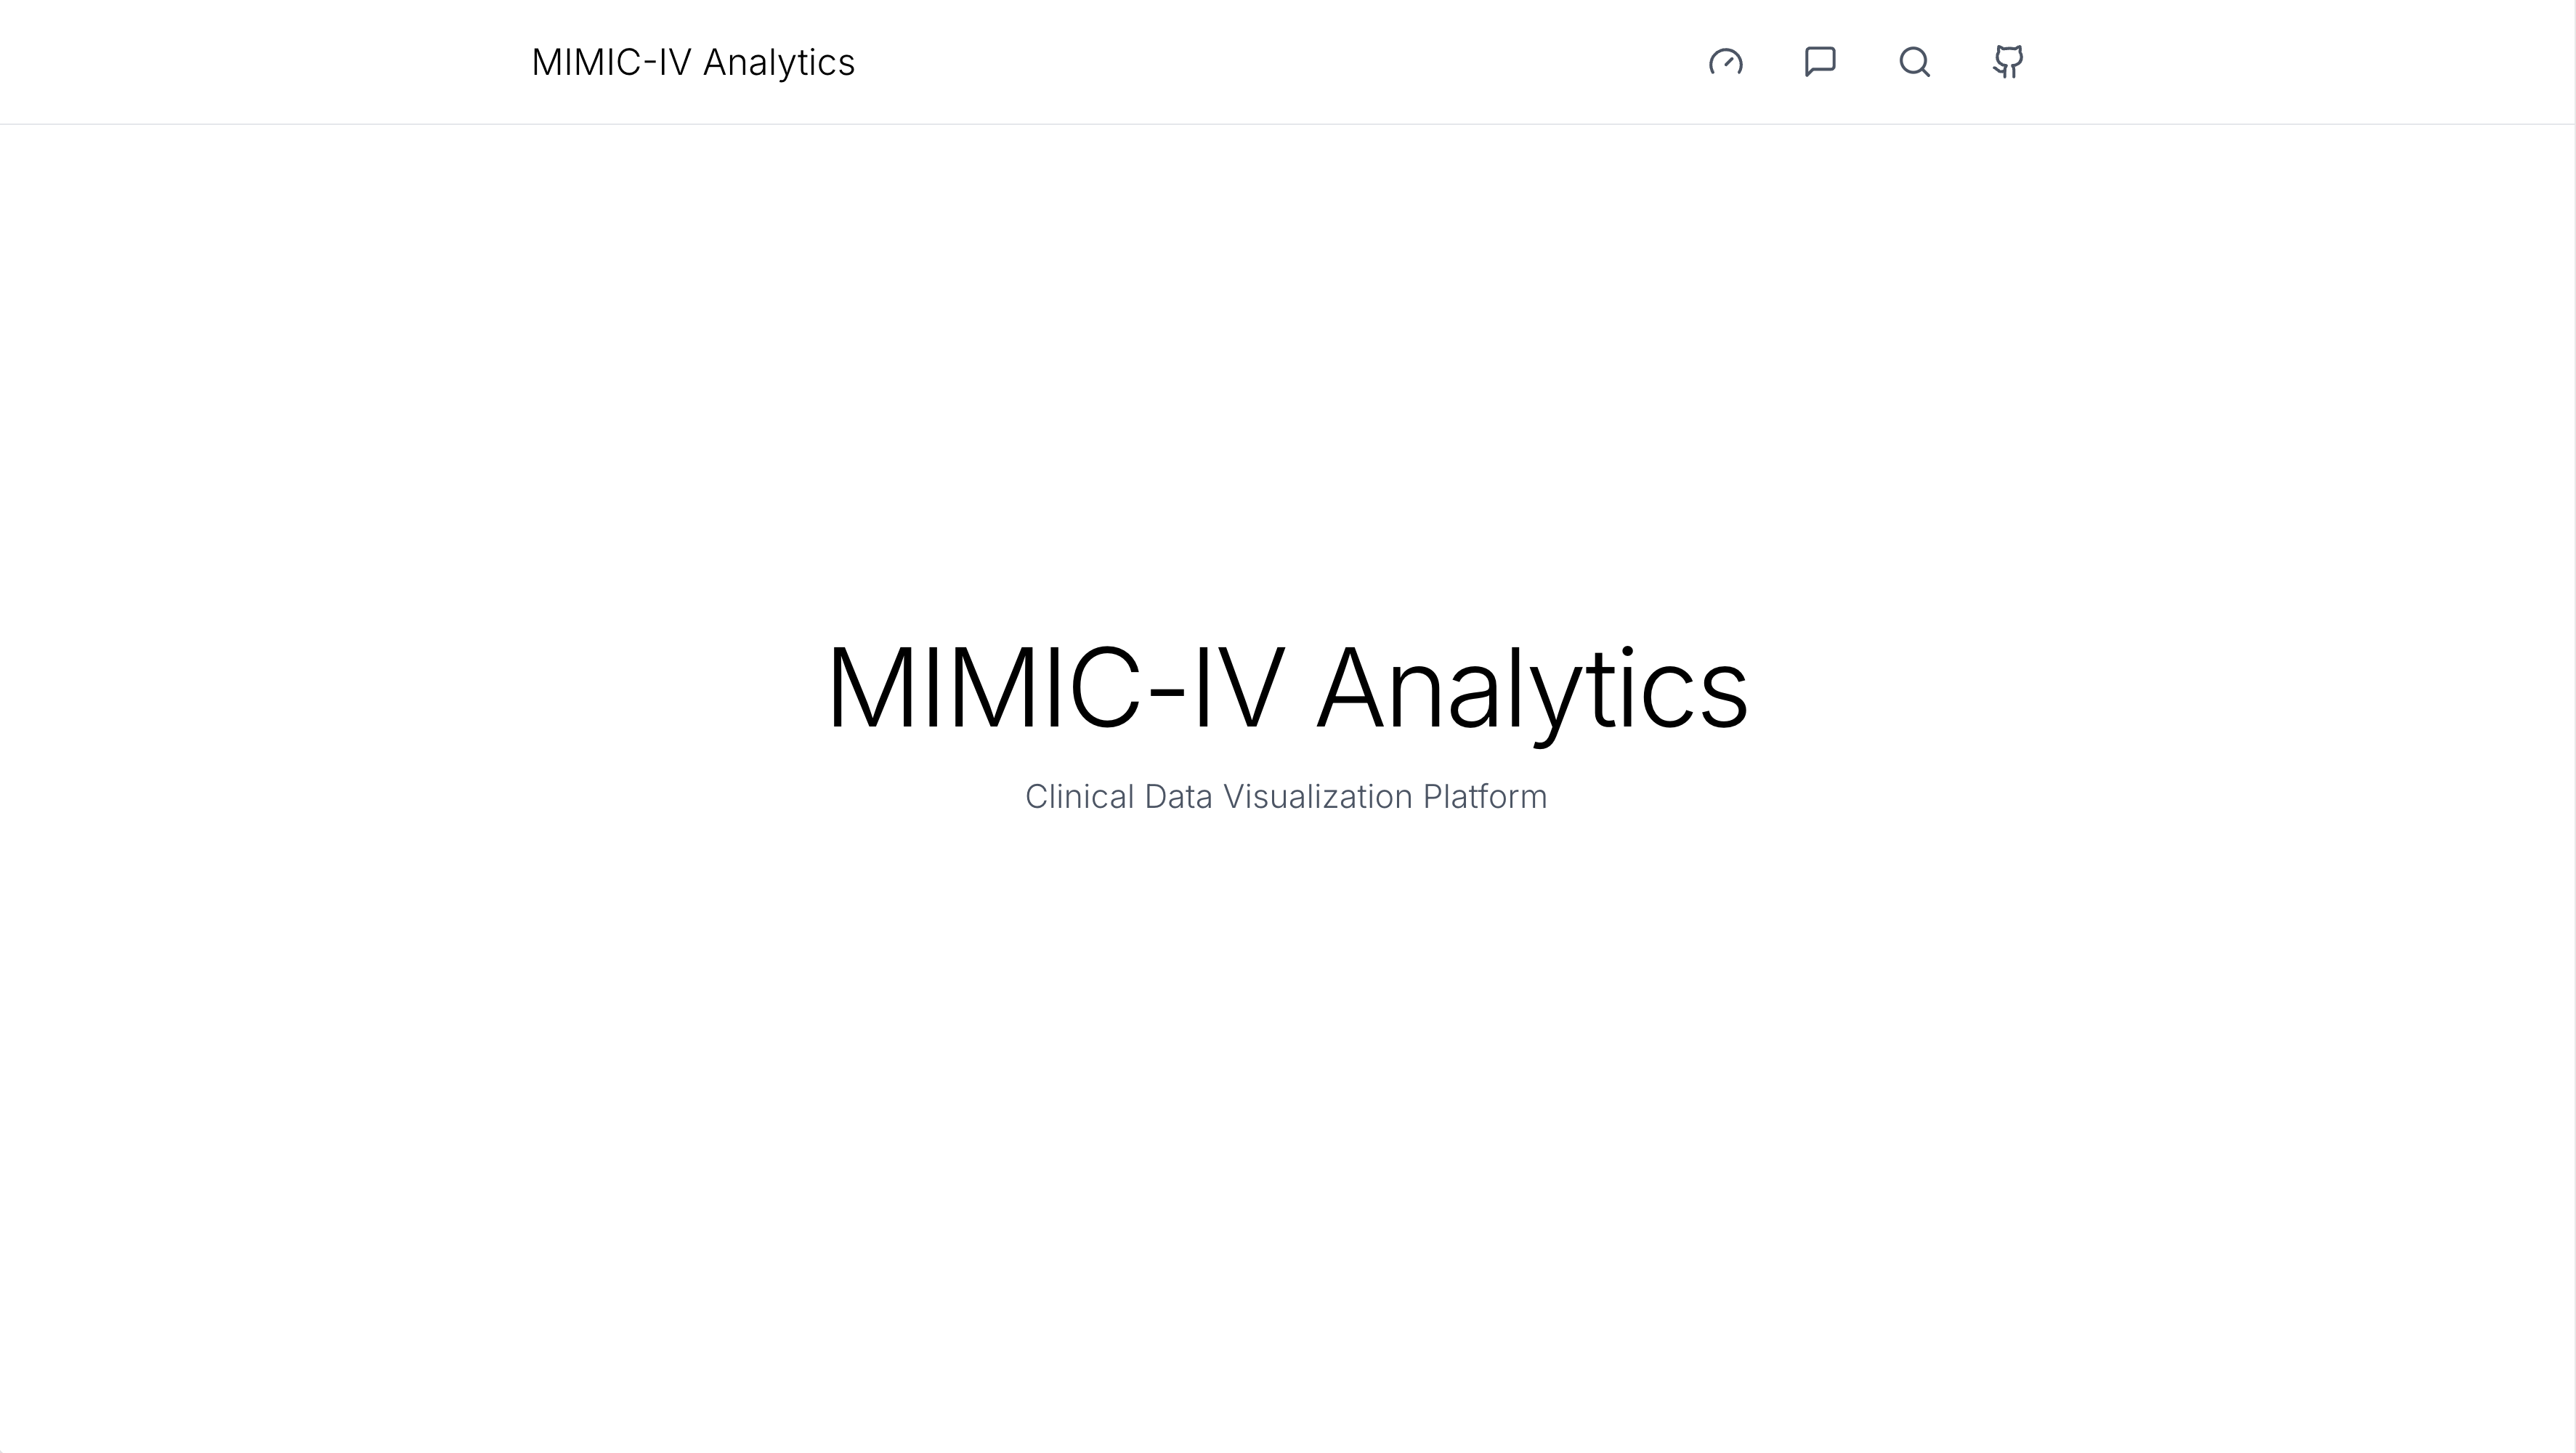
\includegraphics[width=1\textwidth]{imagenes/home.png}}
  \caption{Captura de pantalla de la página principal.}
  \label{fig:home}
\end{figure}

\subsection{Página del dashboard}
El objetivo de esta página es ofrecer al usuario una visión clara y accesible de las estadísticas más relevantes de la base de datos, seleccionadas por su importancia clínica. Para facilitar la interpretación y mejorar la experiencia de usuario, toda la información de MIMIC-IV se ha organizado en cinco grandes categorías: Demográficos y Admisiones, Cuidados Intensivos, Laboratorio y Medicamentos, Diagnósticos y Procedimientos, y Flujos Hospitalarios. En cada una de estas categorías se presentan tres indicadores estadísticos destacados, junto con enlaces a las visualizaciones asociadas. En total, se han implementado seis visualizaciones: dos para la categoría de Demográficos y Admisiones, y una para cada una de las categorías restantes.

En un entorno médico real e ideal, estos datos se actualizarían dinámicamente, permitiendo monitorizar de un vistazo los principales KPIs (Key Performance Indicators) y facilitando la toma de decisiones. Esta página sienta las bases para desarrollos futuros, en los que los profesionales sanitarios podrían filtrar los datos por periodos de tiempo, realizar comparativas o explorar tendencias, obteniendo así información relevante y actualizada sobre el estado del hospital. 
\begin{figure}[H]
  \centering
  \fbox{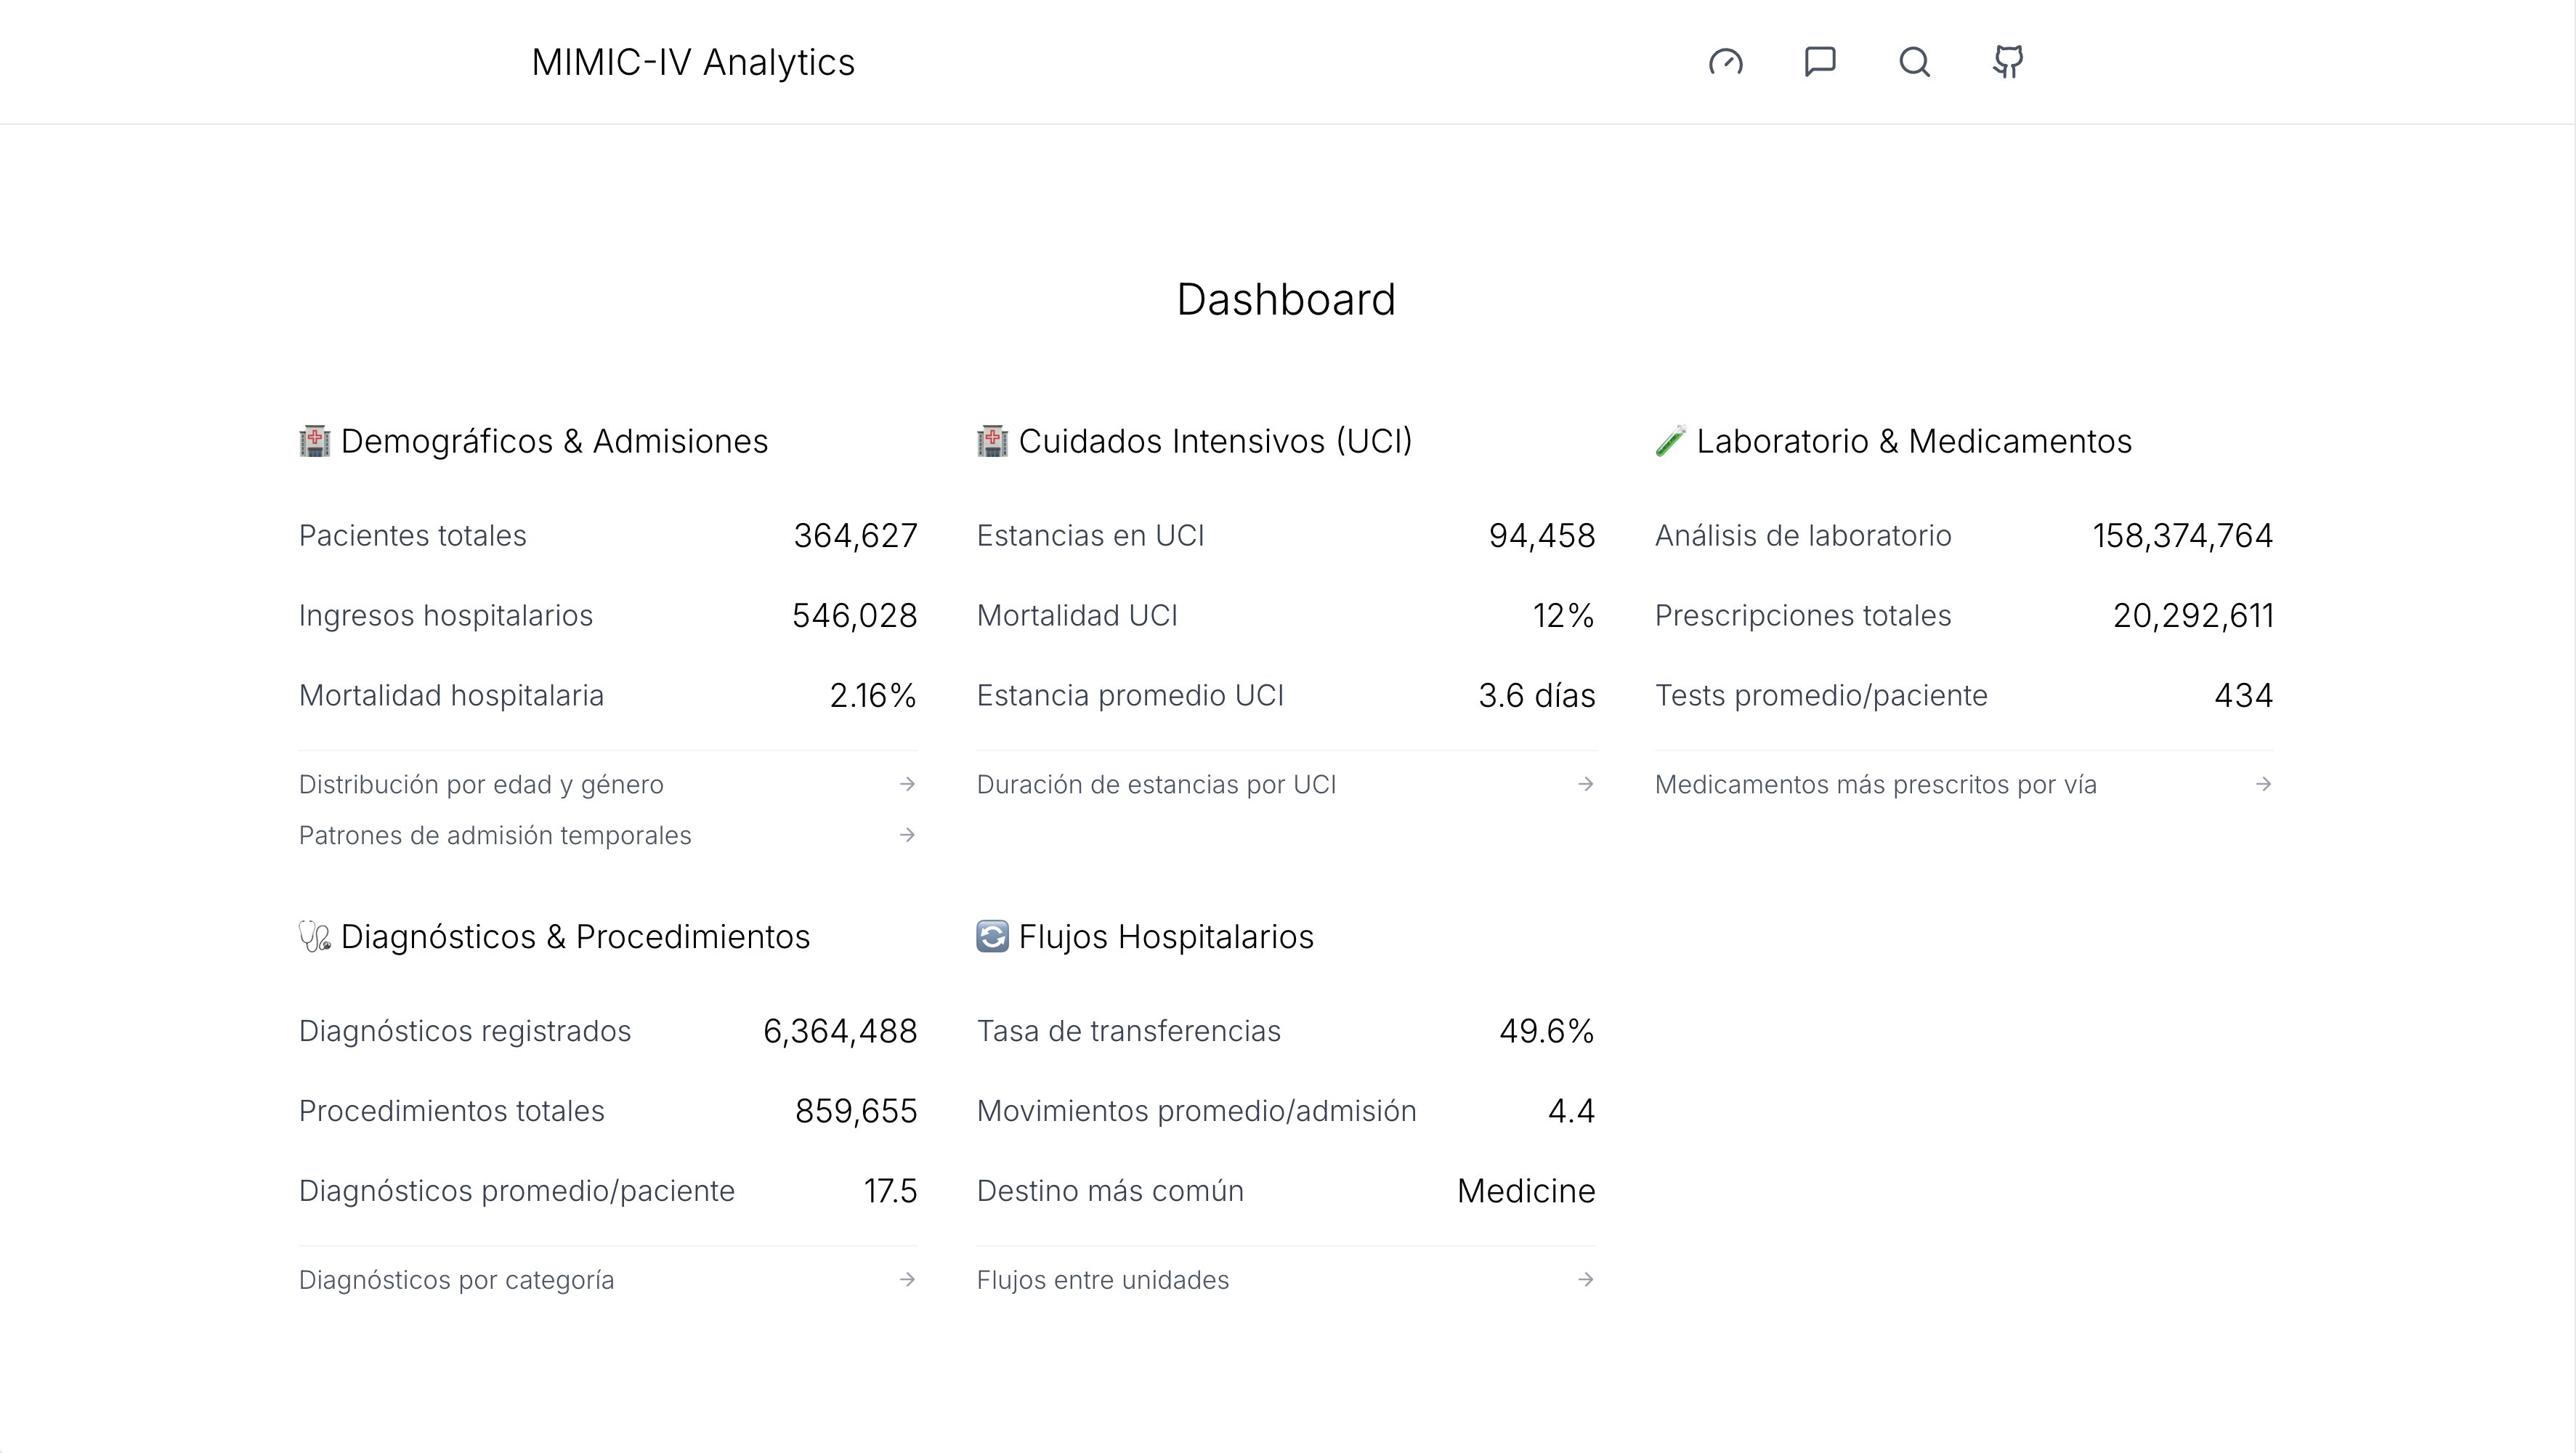
\includegraphics[width=1\textwidth]{imagenes/dash.png}}
  \caption{Captura de pantalla de la página del dashboard.}
  \label{fig:dash}
\end{figure}

\subsection{Página del chat}
Para la página del chat se sigue con la estética visual minimalista ya establecida, y se implementa la conexión con el backend, que ejecuta toda la lógica de comunicación entre el LLM, la base de datos gracias al protocolo MCP, y el frontend.
\begin{figure}[H]
  \centering
  \fbox{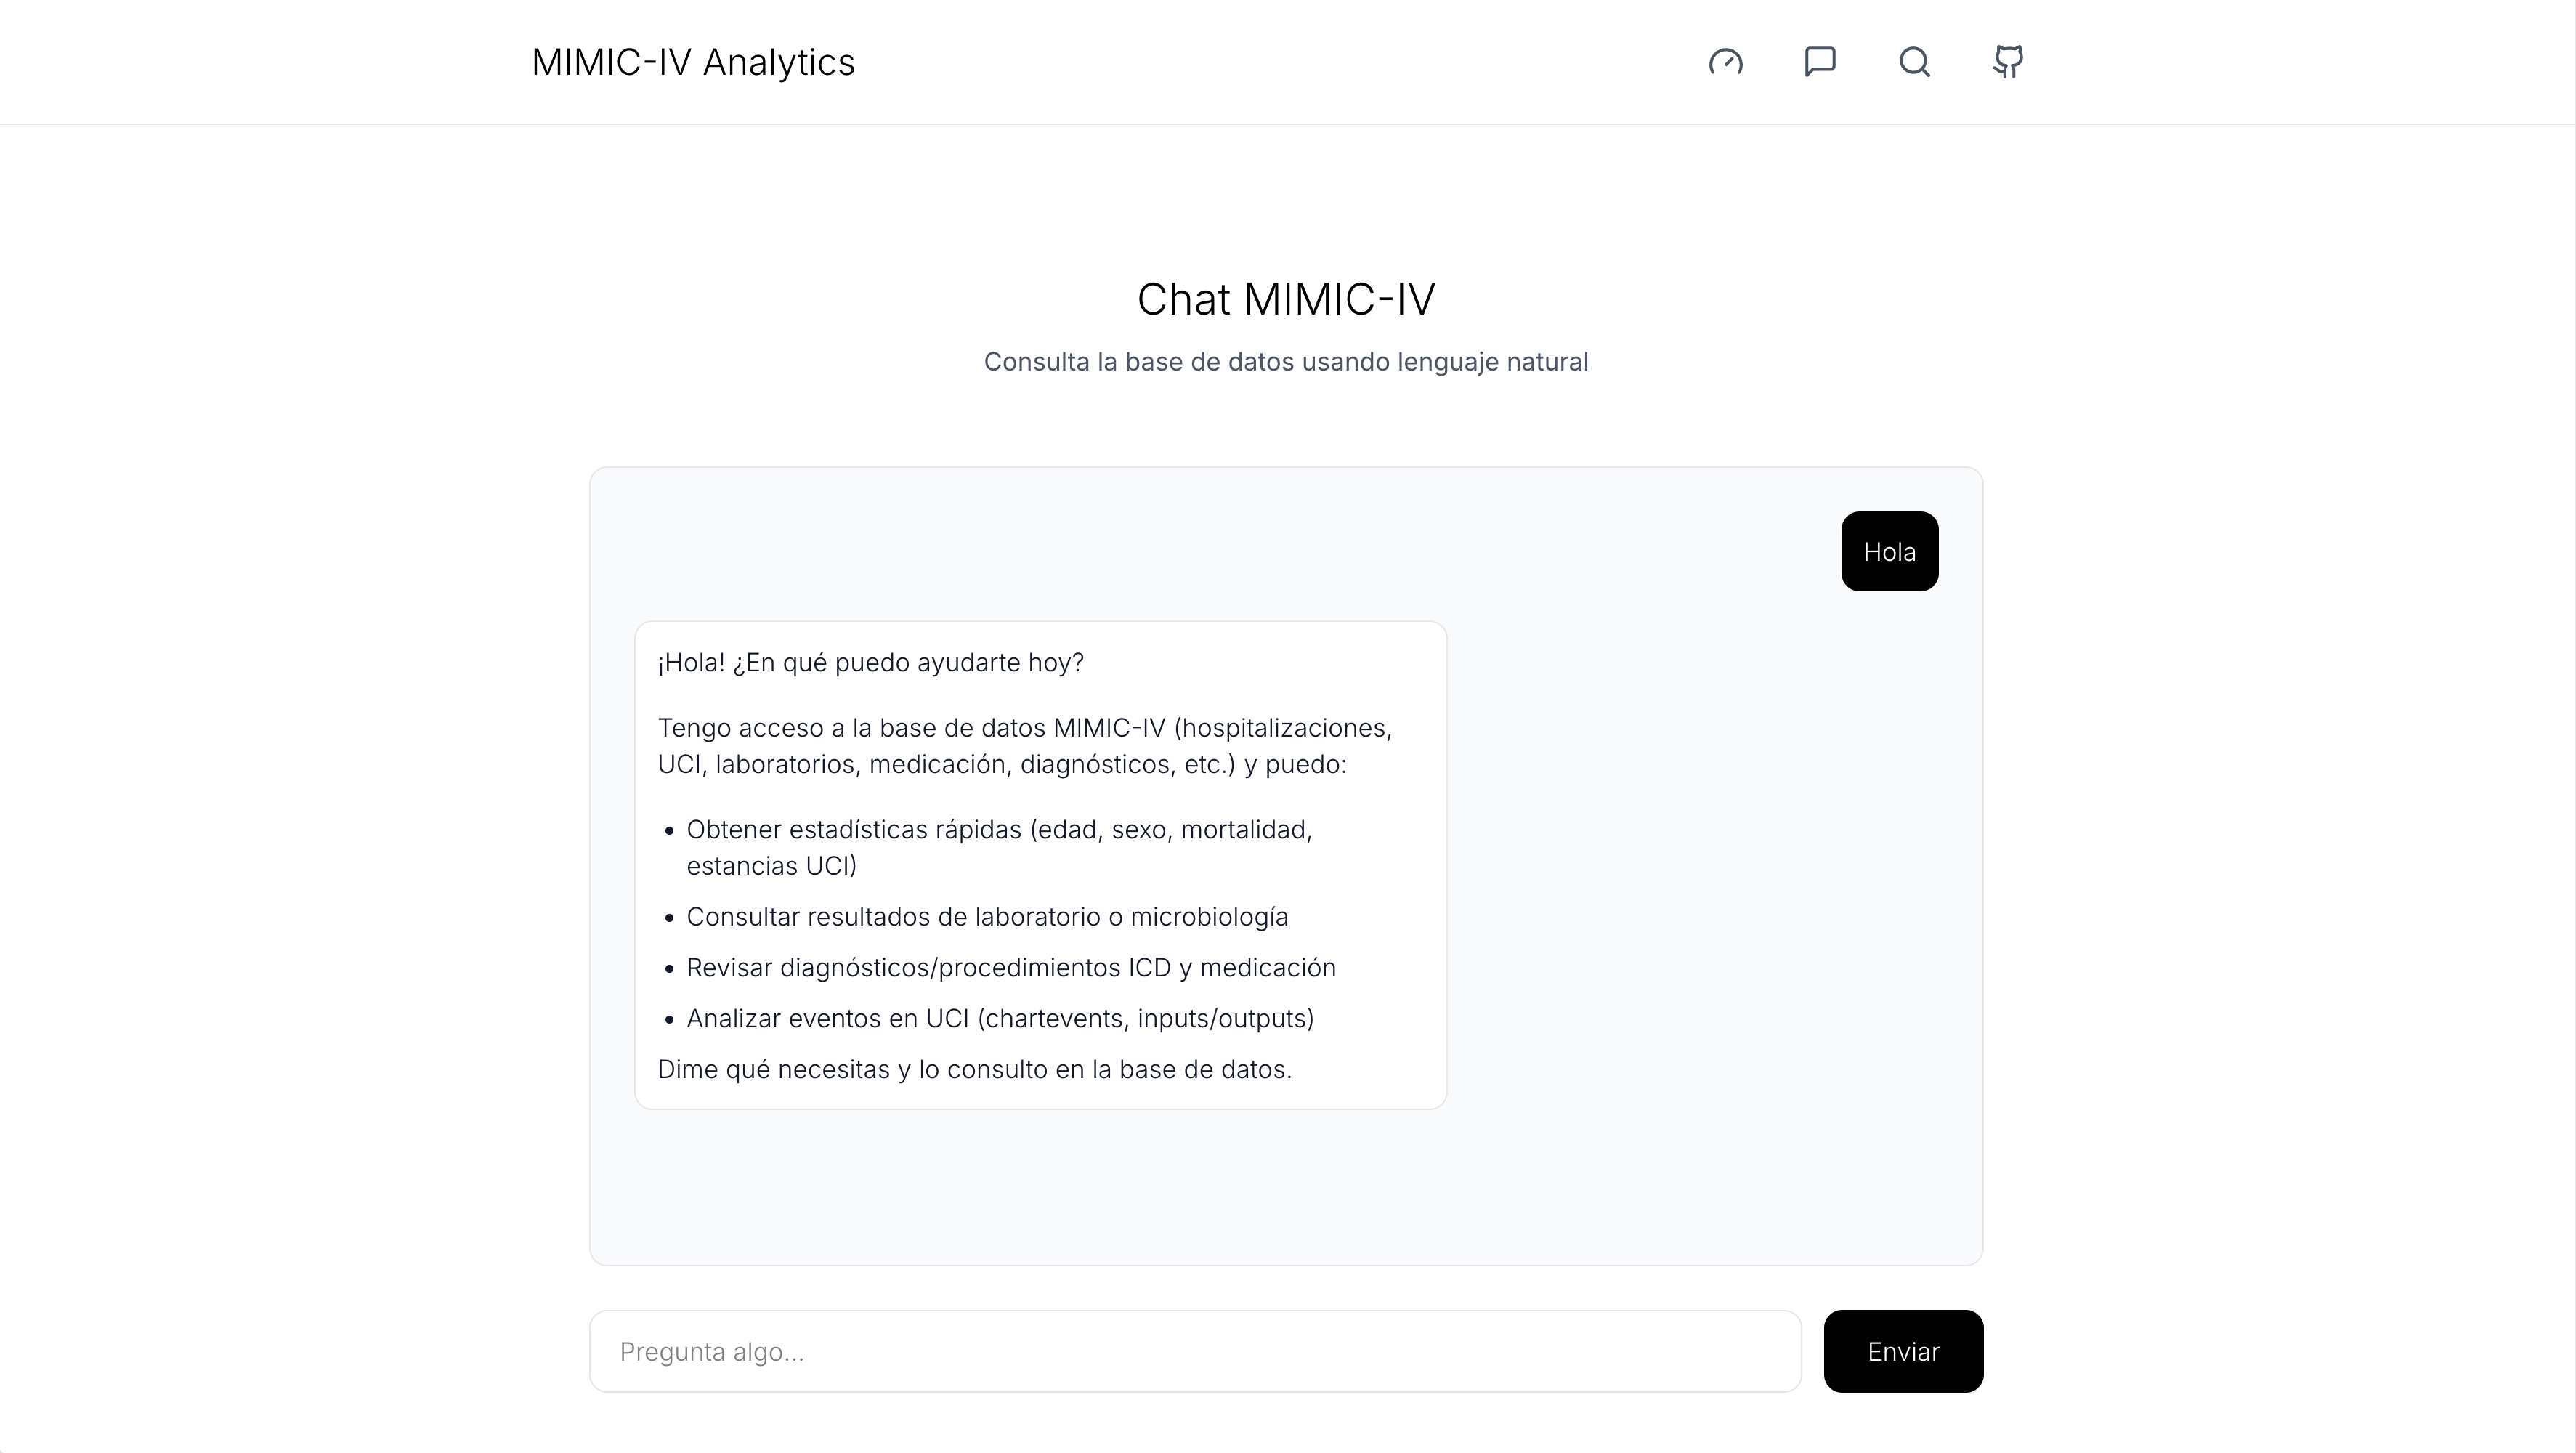
\includegraphics[width=1\textwidth]{imagenes/chat.png}}
  \caption{Captura de pantalla de la página del chat.}
  \label{fig:chat}
\end{figure}

\subsection{Página de búsqueda de pacientes}
Esta sencilla página nos permite comprobar la existencia de un paciente mediante su identificador único, mediante llamadas al endpoint del backend \texttt{/api/patients/\$\{id\}/exists}, y si es así (obtenemos status code 200 OK) entonces redirigimos a la página individual del paciente \texttt{/patient/\$\{id\}}. 
\begin{figure}[H]
  \centering
  \fbox{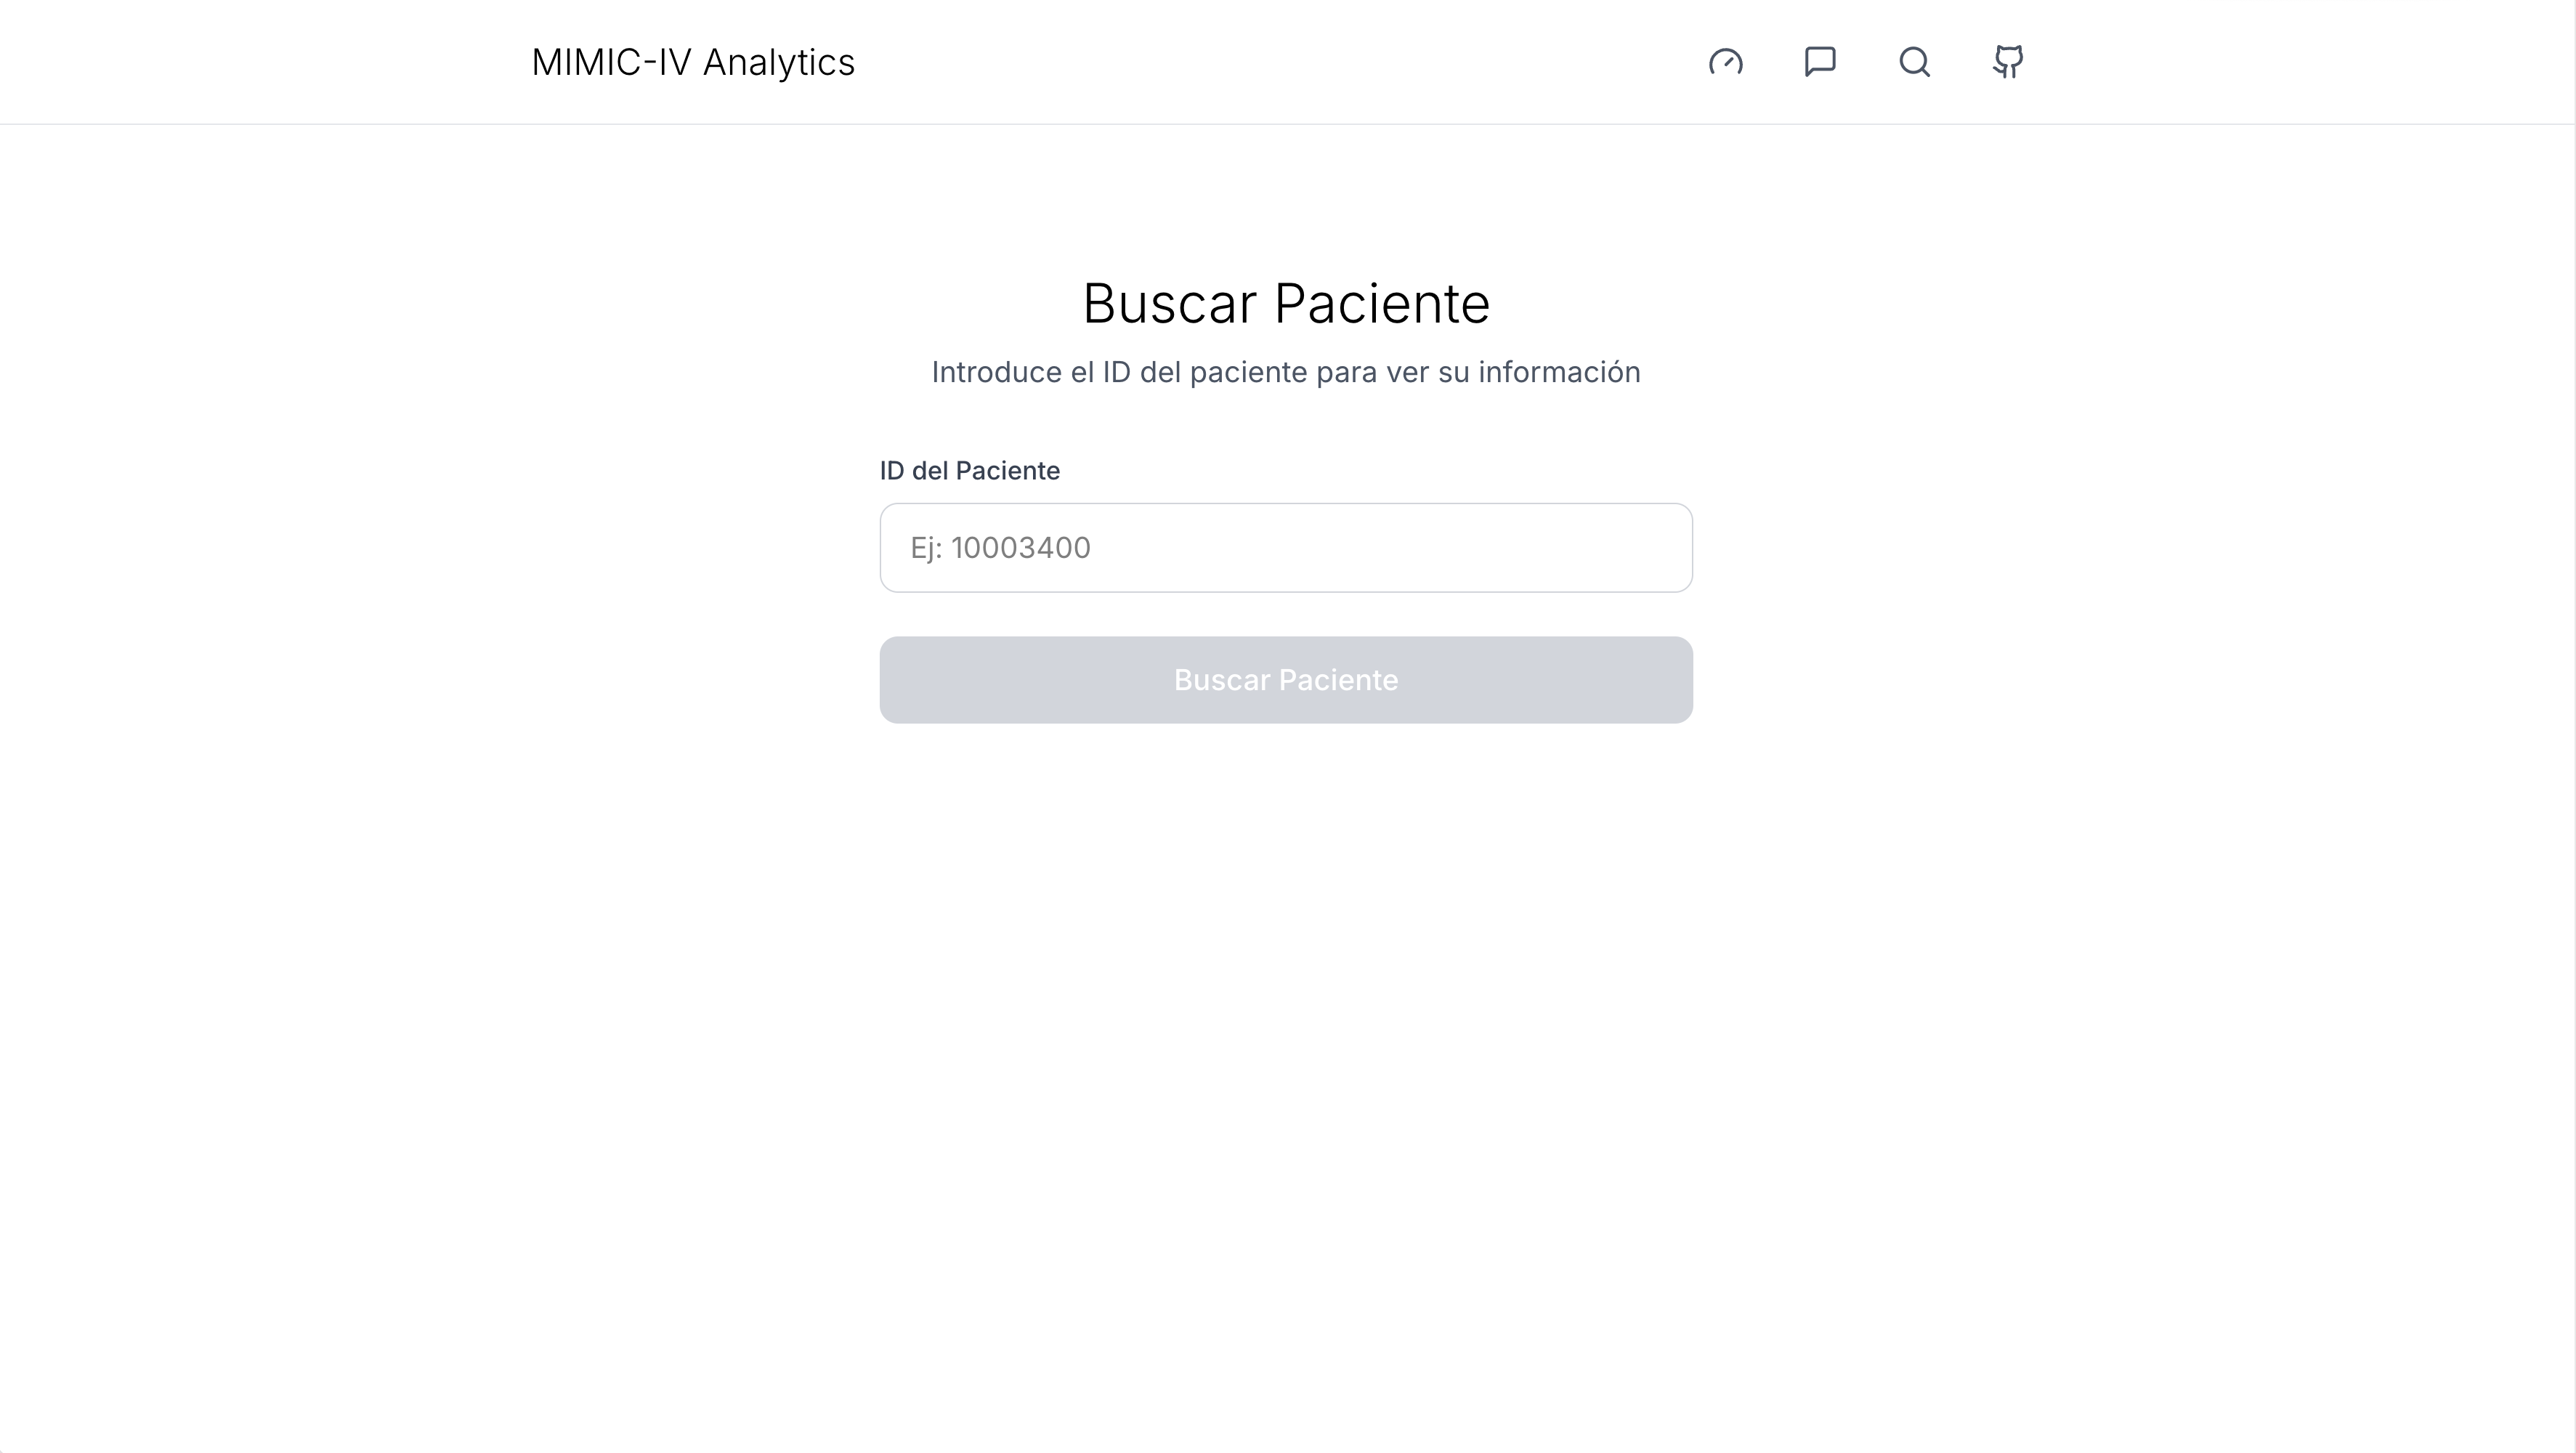
\includegraphics[width=1\textwidth]{imagenes/search.png}}
  \caption{Captura de pantalla de la página de búsqueda de pacientes.}
  \label{fig:search}
\end{figure}

\subsection{Página del paciente individual}
Al aterrizar en una de estas páginas, lo que hacemos es obtener el ID del paciente (\texttt{subject\_id}) de la URL, y lo envíamos al backend, a la ruta \texttt{/api/patients/\$\{id\}}. Este nos devuelve absolutamente toda la información relacionada con el paciente que necesitamos, por lo que puede tardar varios segundos en responder. Una vez con los datos, los mostramos de forma estructurada y visualmente agradable. A continuación se explican las tres secciones distintas en las que se ha organizado la información, las cuales han sido implementadas como componentes distintos que reciben los datos que necesitan de la página padre.

En primer lugar encontramos una sección con la información demográfica básica del paciente: género, edad, idioma, raza, etc. Implementado en el componente React \texttt{PatientBasicInfo}.

En segundo lugar, una sección con un resumen del historial del paciente generado mediante Inteligencia Artificial, que sintetiza diagnósticos y procedimientos relevantes a partir de los datos de la ficha.

En tercer lugar tenemos el grueso de la información, en el componente \texttt{PatientAdmissions}. En el mediante desplegables, vemos un listado de todos los ingresos que ha tenido el paciente, junto a algunas estadísticas rápidas para ver a simple vista: número de días de duración de la hospitalización, número de diagnósticos asociados a la estancia, número de procedimientos, y número de tests de laboratorio. 

Al hacer click en el desplegable, podemos ver más información del ingreso, como las fechas exactas de entrada y salida, el tipo del seguro del paciente, a dónde se trasfirió despues, etc. Además, de nuevo, a forma de desplegables, podemos ver la información detallada de los diagnósticos, procedimientos, y tests de laboratorio.

En cuanto a los últimos, es posible filtrar los tests por categoría (Blood Gas, Hematology, Chemistry...) o verlos todos, y al seleccionar un test con varias ocurrencias se presenta una serie temporal que facilita observar la evolución clínica.
\begin{figure}[H]
  \centering
  \fbox{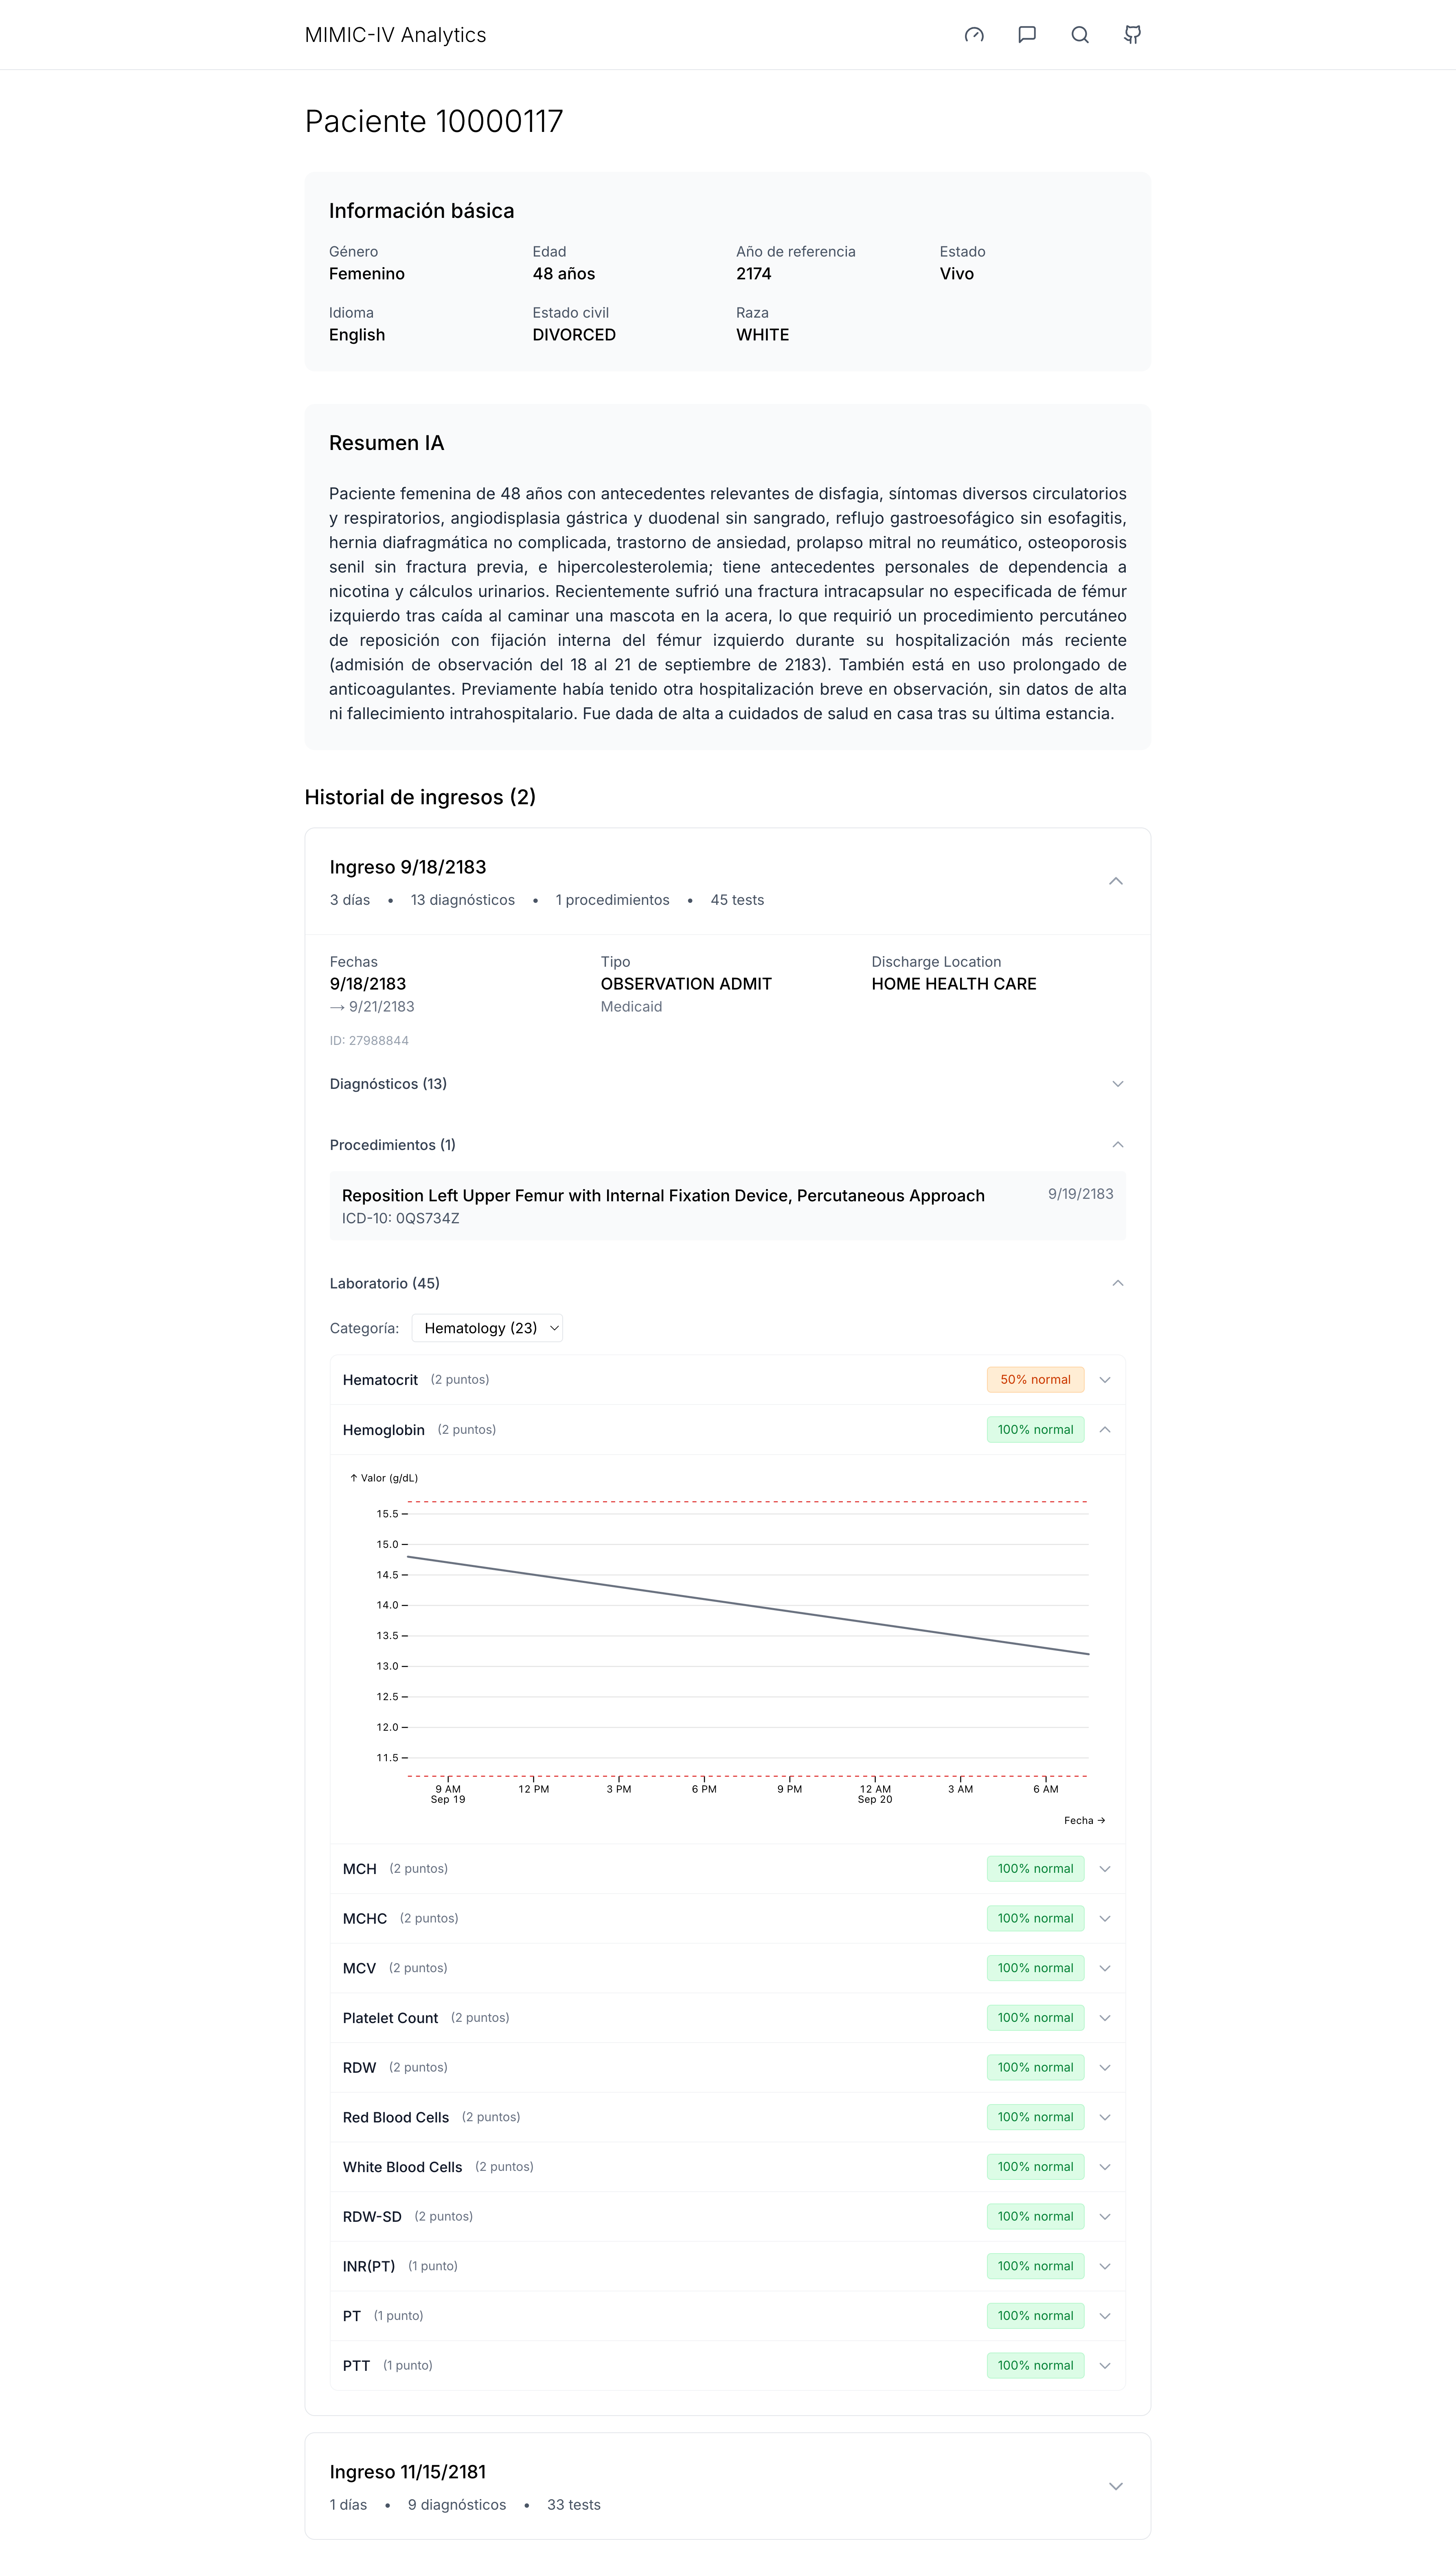
\includegraphics[width=0.9\textwidth]{imagenes/patient1.png}}
  \caption{Captura de pantalla de la página del paciente.}
  \label{fig:patient}
\end{figure}

\section{Visualizaciones y lectura}
En esta sección se muestran ejemplos concretos de la aplicación y una breve interpretación de cada visualización, centrada en lo que revela el dato en este contexto específico.

\subsection{Distribución por edad y género}
Ahora vamos a pasar a las visualizaciones de datos que se han implementado. El primer gráfico, realizado utilizando Observable Plot, es un Population Pyramid \cite{populationPyramid} de la distribución por edad y género, con dos variantes, una por rangos de edad, y la otra por edad específica.
\begin{figure}[H]
  \centering
  \fbox{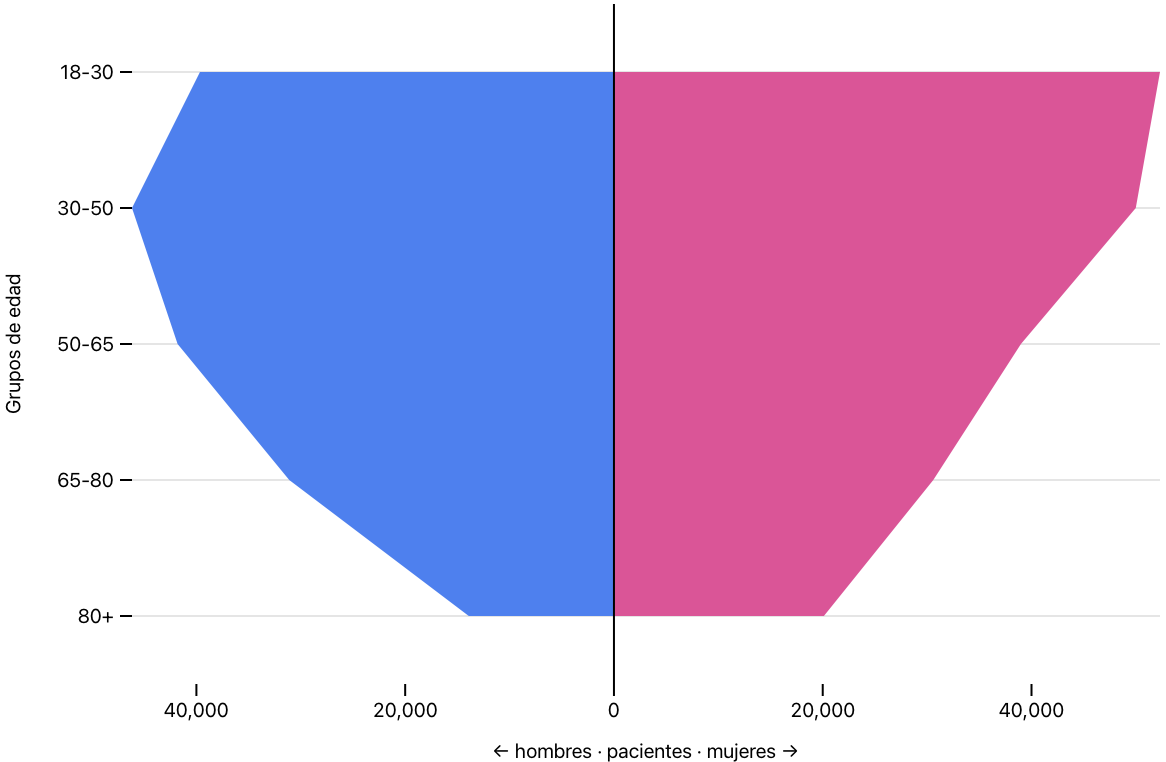
\includegraphics[width=0.65\textwidth]{imagenes/chart2.png}}
  \caption{Distribución por edad y género (rangos de edad)}
  \label{fig:chart2}
\end{figure}
\begin{figure}[H]
  \centering
  \fbox{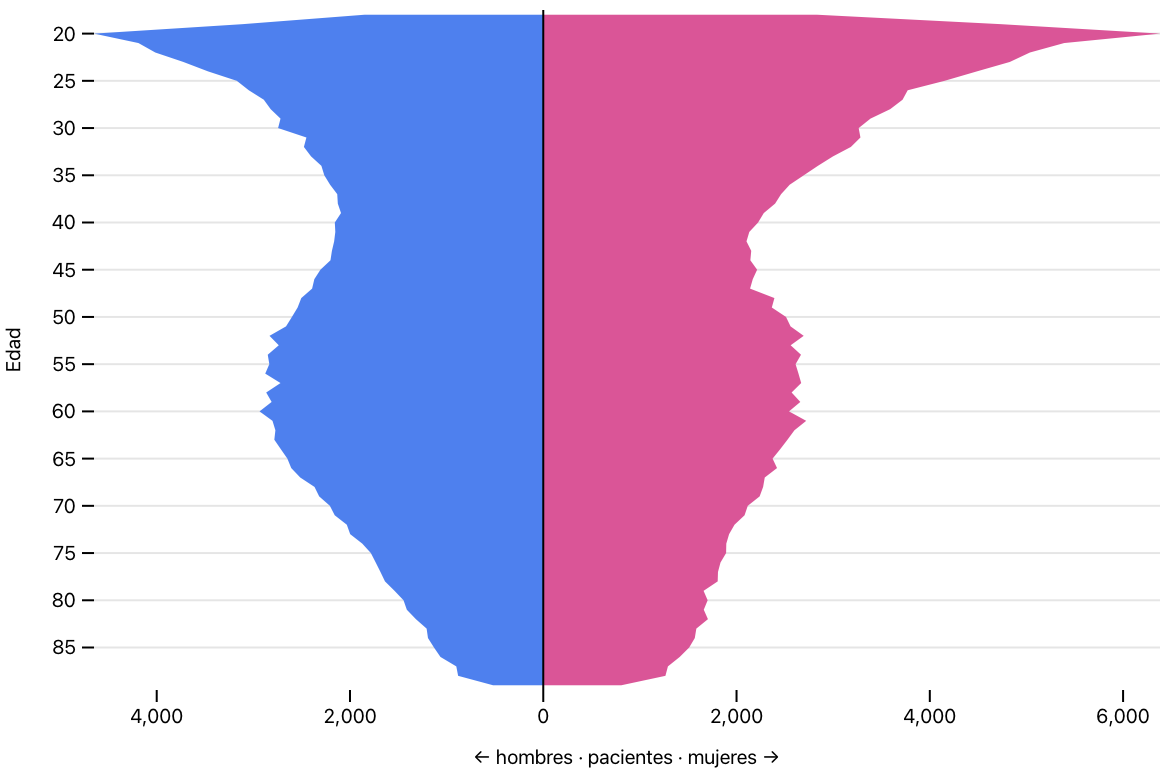
\includegraphics[width=0.65\textwidth]{imagenes/chart3.png}}
  \caption{Distribución por edad y género}
  \label{fig:chart3}
\end{figure}

\subsection{Heatmap de ingresos}
El segundo gráfico, desarrollado con Observable Plot, representa la cantidad de ingresos por hora/día de la semana y por mes/día del mes. En la vista horaria se aprecian franjas de mayor actividad y posibles cambios de turno; en la vista mensual se observan patrones estacionales o días con menor actividad relativa. La interpretación se centra en localizar picos y valles consistentes.
\begin{figure}[H]
  \centering
  \fbox{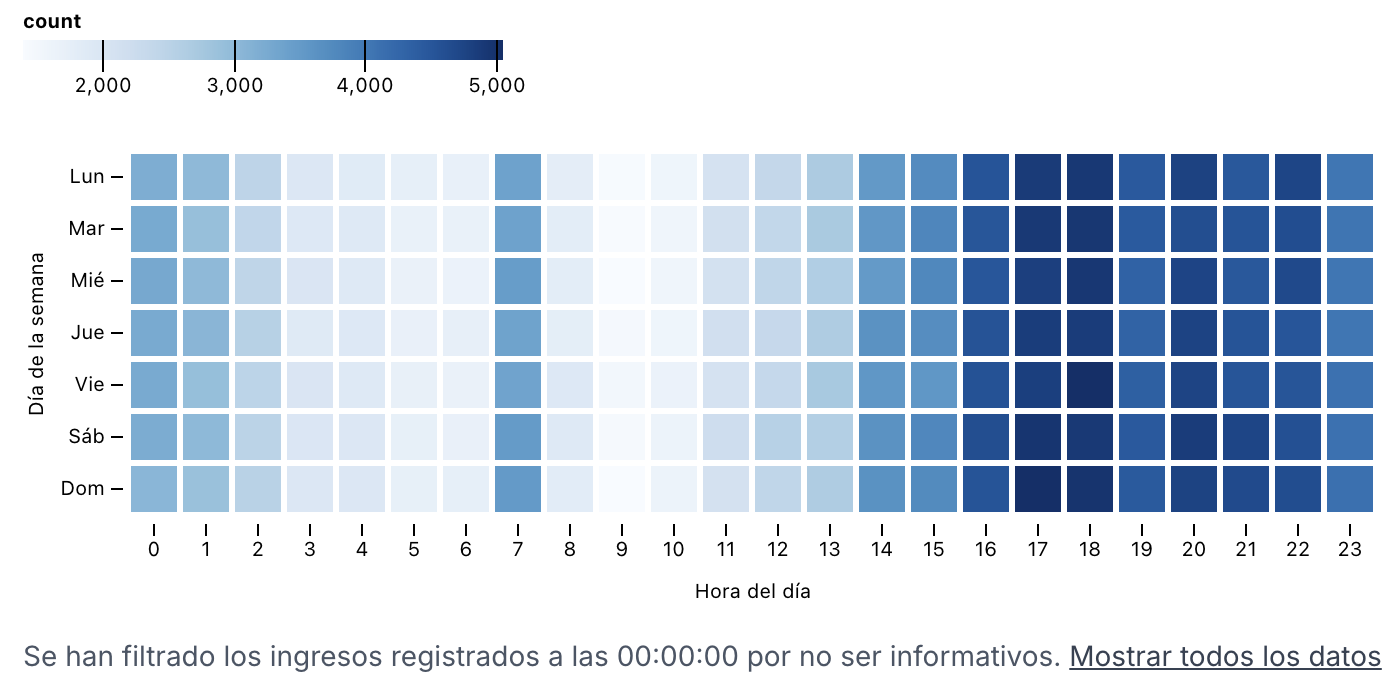
\includegraphics[width=0.8\textwidth]{imagenes/chart-heat-1.png}}
  \caption{Heatmap de ingresos por hora y día de la semana.}
  \label{fig:chart-heat-1}
\end{figure}
\begin{figure}[H]
  \centering
  \fbox{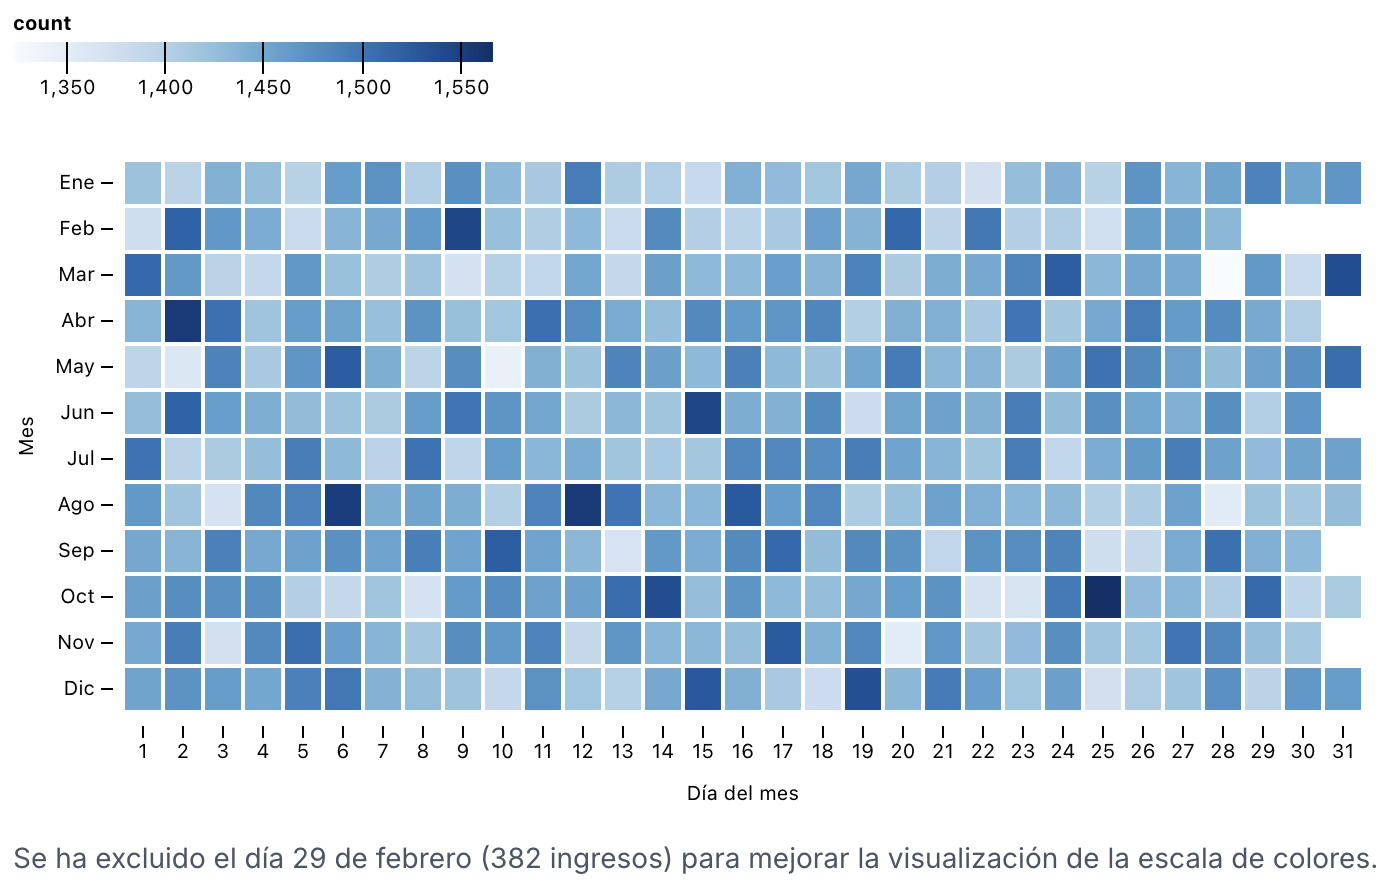
\includegraphics[width=0.8\textwidth]{imagenes/chart-heat-2.png}}
  \caption{Heatmap de ingresos por mes y día del mes.}
  \label{fig:chart-heat-2}
\end{figure}

\subsection{Estancia promedio por unidad UCI}
Este gráfico, un Horizontal Bar Chart \cite{hbarchart}, muestra el número de días promedio de estancia por unidad UCI. La lectura comparativa permite identificar unidades con estancias más prolongadas y posibles outliers; conviene considerar el volumen de estancias al contextualizar promedios extremos.
\begin{figure}[H]
  \centering
  \fbox{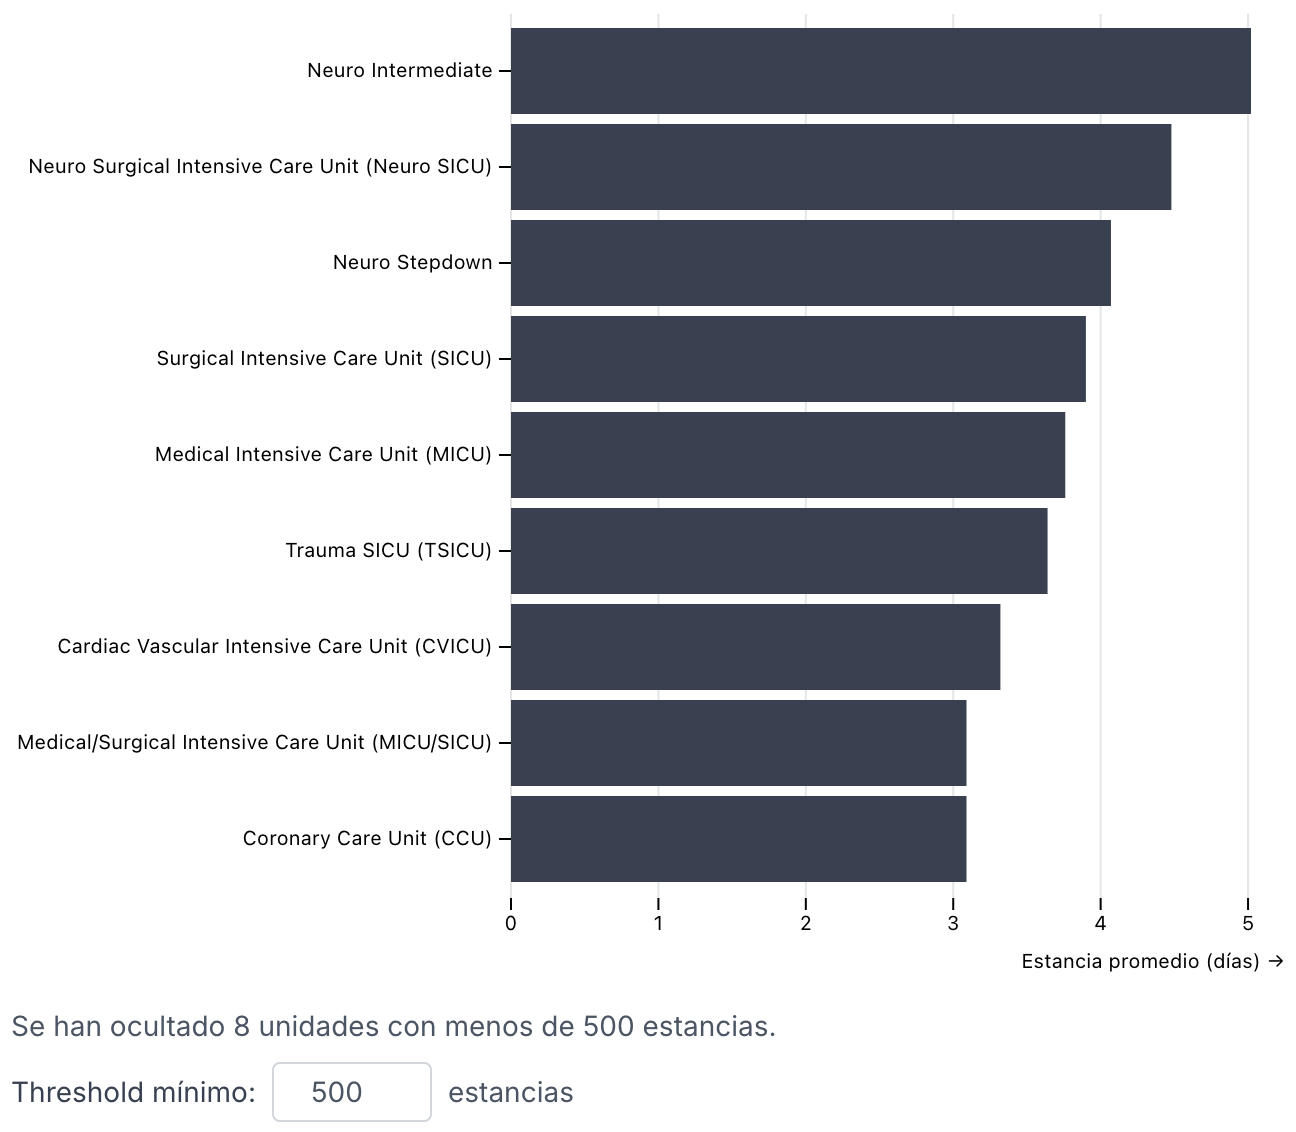
\includegraphics[width=0.75\textwidth]{imagenes/chart-icu.png}}
  \caption{Estancia promedio por unidad UCI}
  \label{fig:chart-icu}
\end{figure}

\subsection{Medicamentos más prescritos por vía}
Un sunburst \cite{sunburst} muestra los medicamentos más frecuentes organizados por vía de administración. La interpretación consiste en comparar sectores y subsectores para identificar rutas dominantes y fármacos predominantes en cada ruta.
\begin{figure}[H]
  \centering
  \fbox{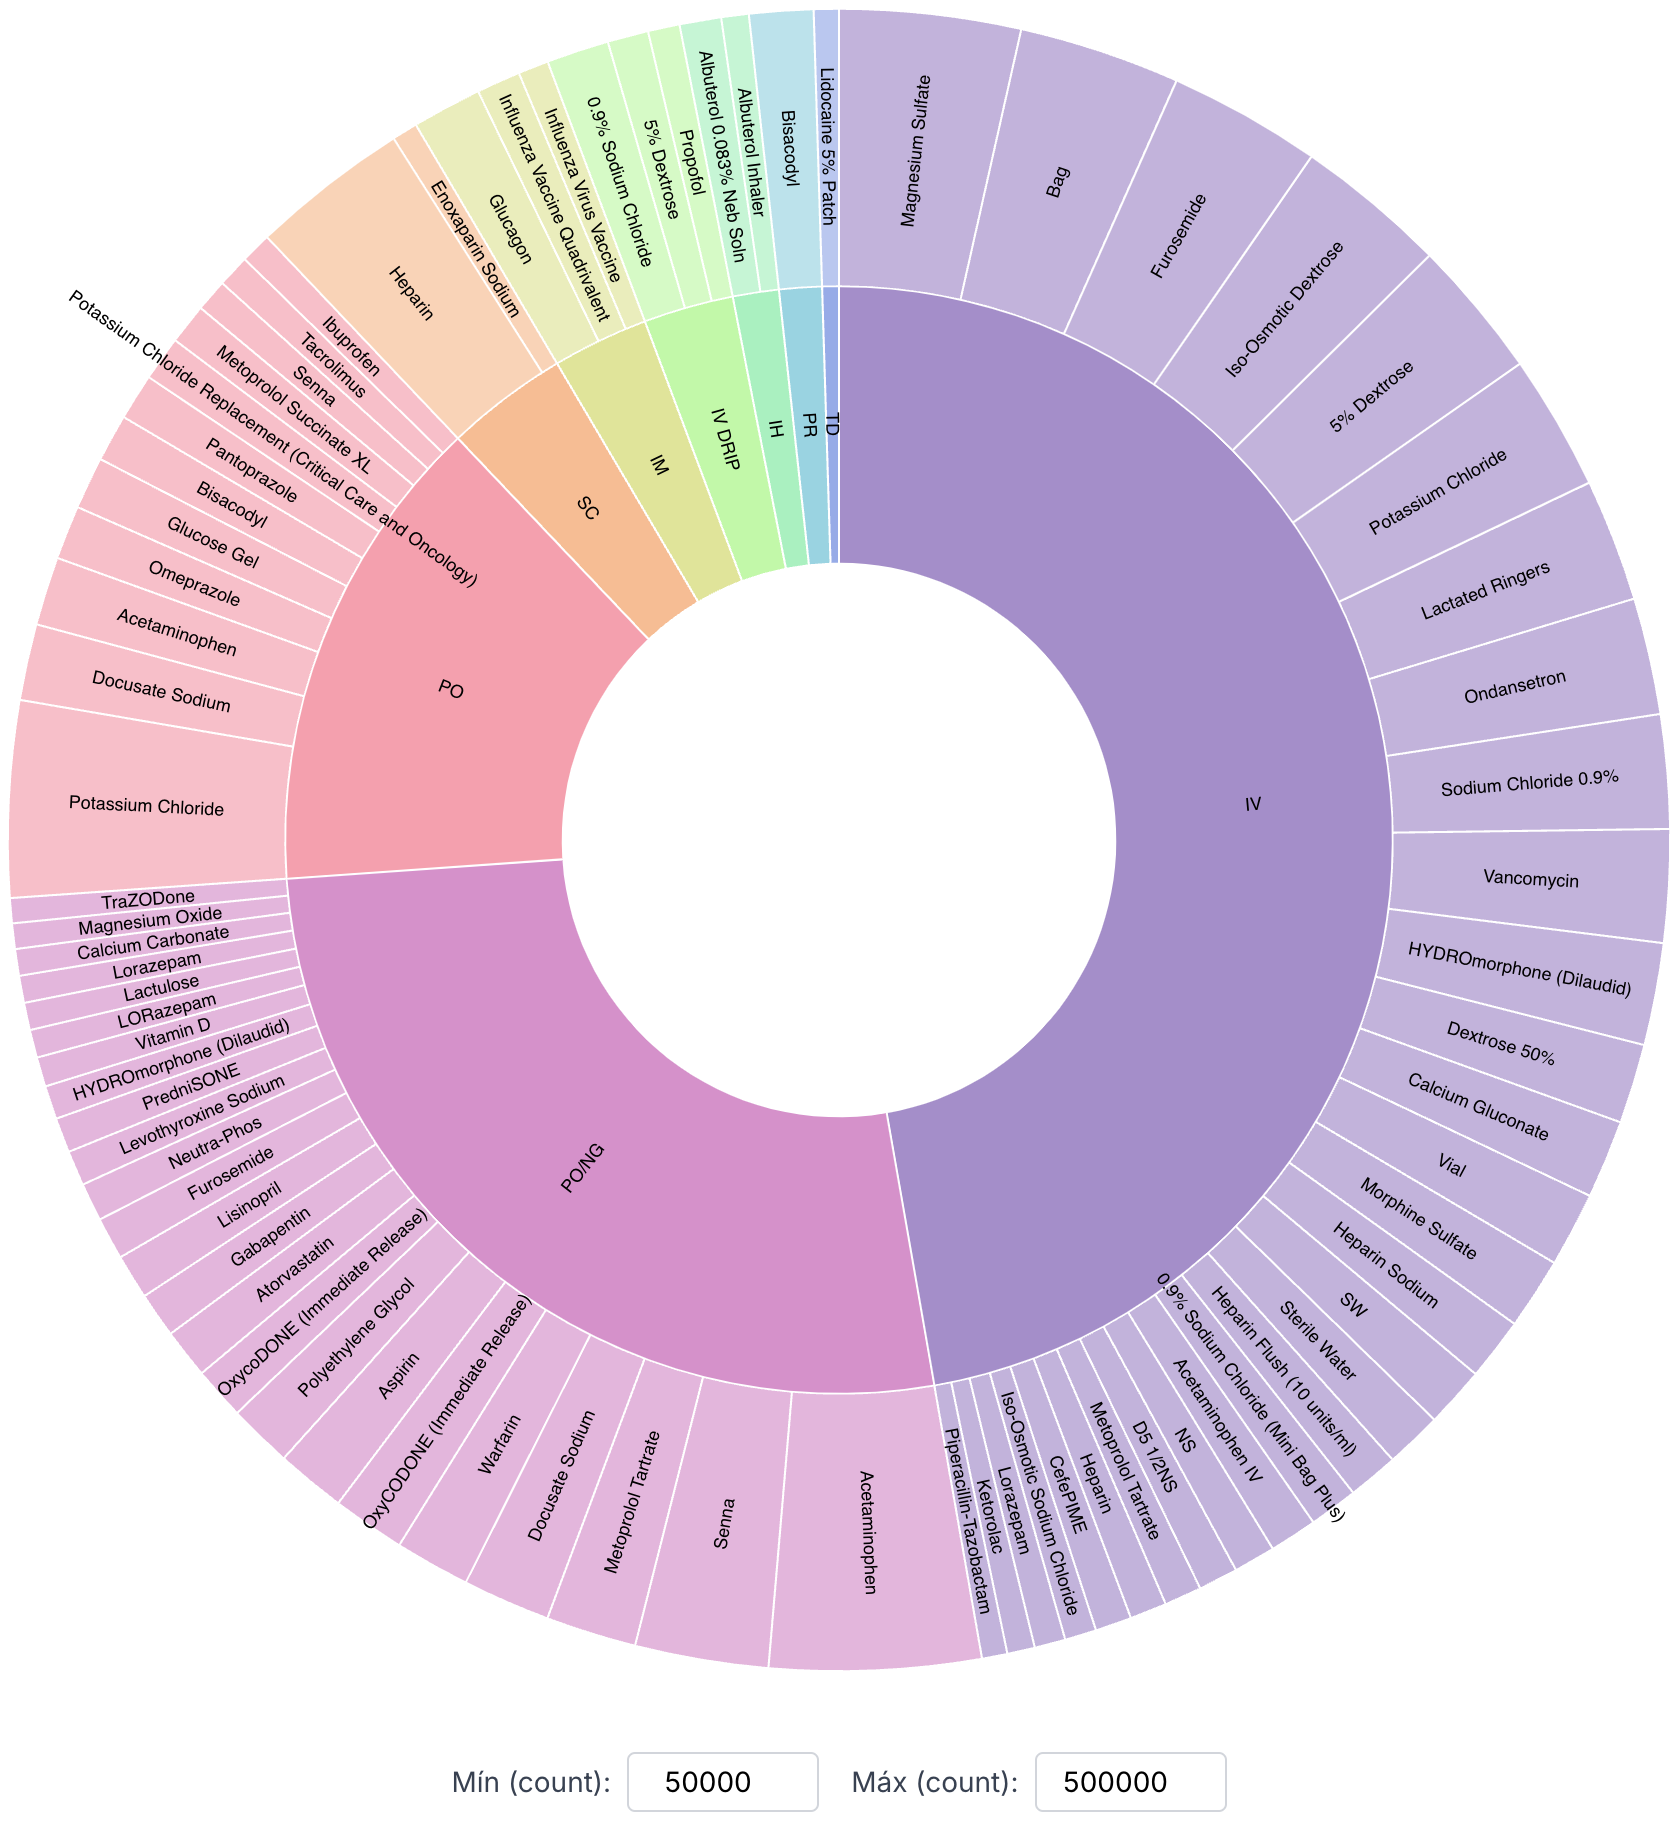
\includegraphics[width=0.85\textwidth]{imagenes/chart-sunburst.png}}
  \caption{Medicamentos más prescritos por vía}
  \label{fig:chart-sunburst}
\end{figure}

\subsection{Diagnósticos por categoría}
Un icicle \cite{icicle} organiza jerárquicamente los diagnósticos según su taxonomía, permitiendo explorar de lo general a lo específico. La lectura se basa en el ancho relativo de cada segmento y en el zoom sobre las ramas de interés para detectar las categorías con mayor prevalencia.
\begin{figure}[H]
  \centering
  \fbox{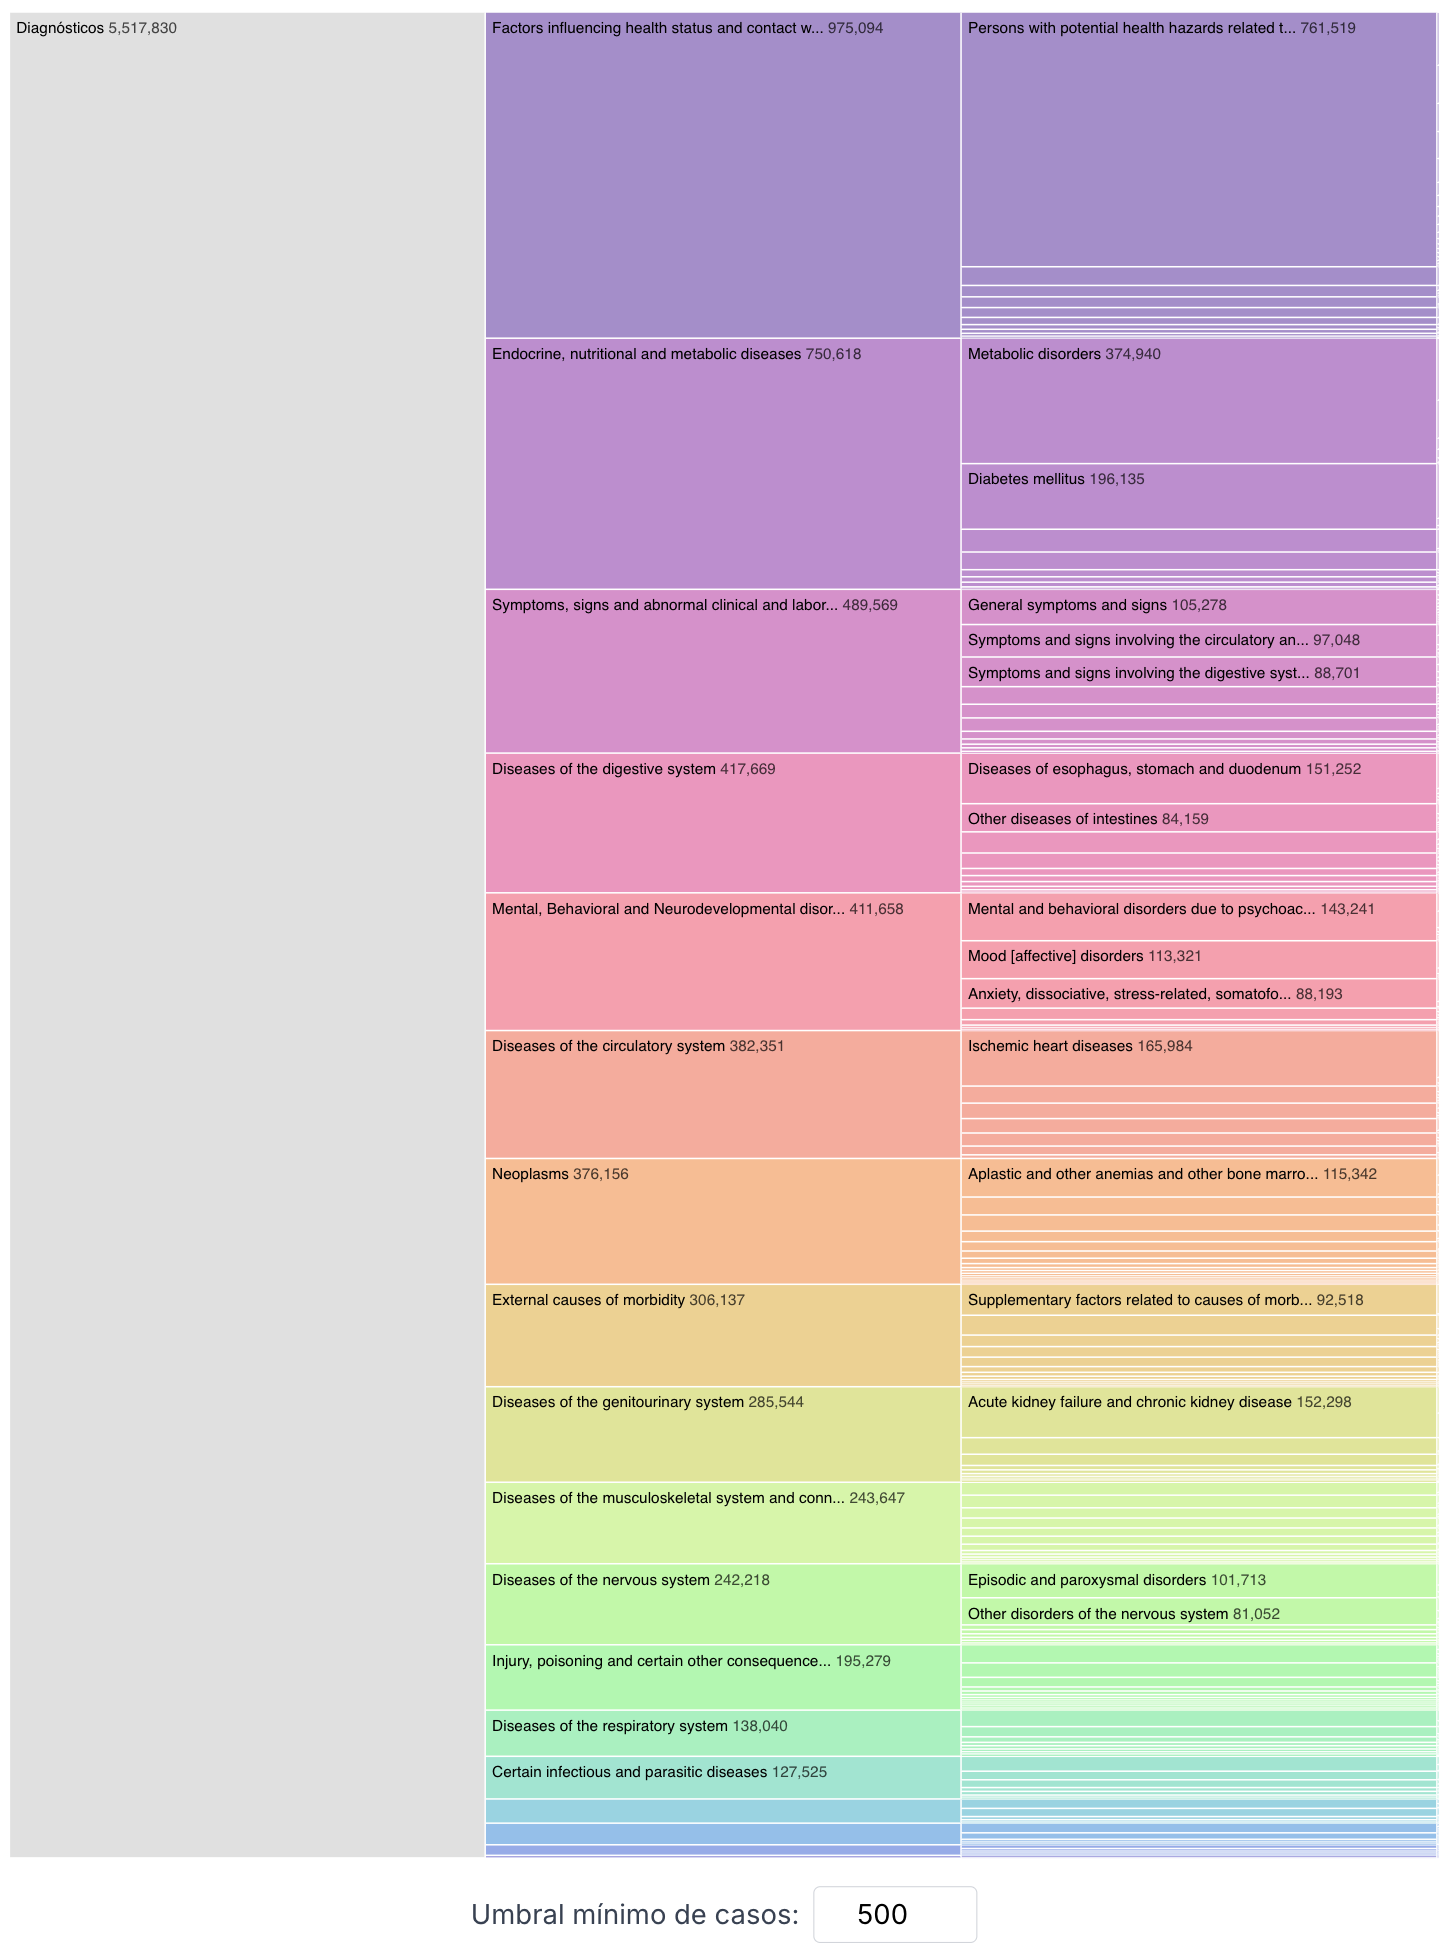
\includegraphics[width=0.88\textwidth]{imagenes/chart-diag.png}}
  \caption{Diagnósticos por categoría}
  \label{fig:chart-diag}
\end{figure}

\subsection{Flujos hospitalarios}
Un directed chord diagram \cite{chord} presenta las transferencias entre unidades; la dirección y el grosor de los acordes permiten identificar orígenes, destinos y relaciones dominantes. La interpretación se centra en los pares con mayor flujo y en asimetrías notables entre ida y vuelta.
\begin{figure}[H]
  \centering
  \fbox{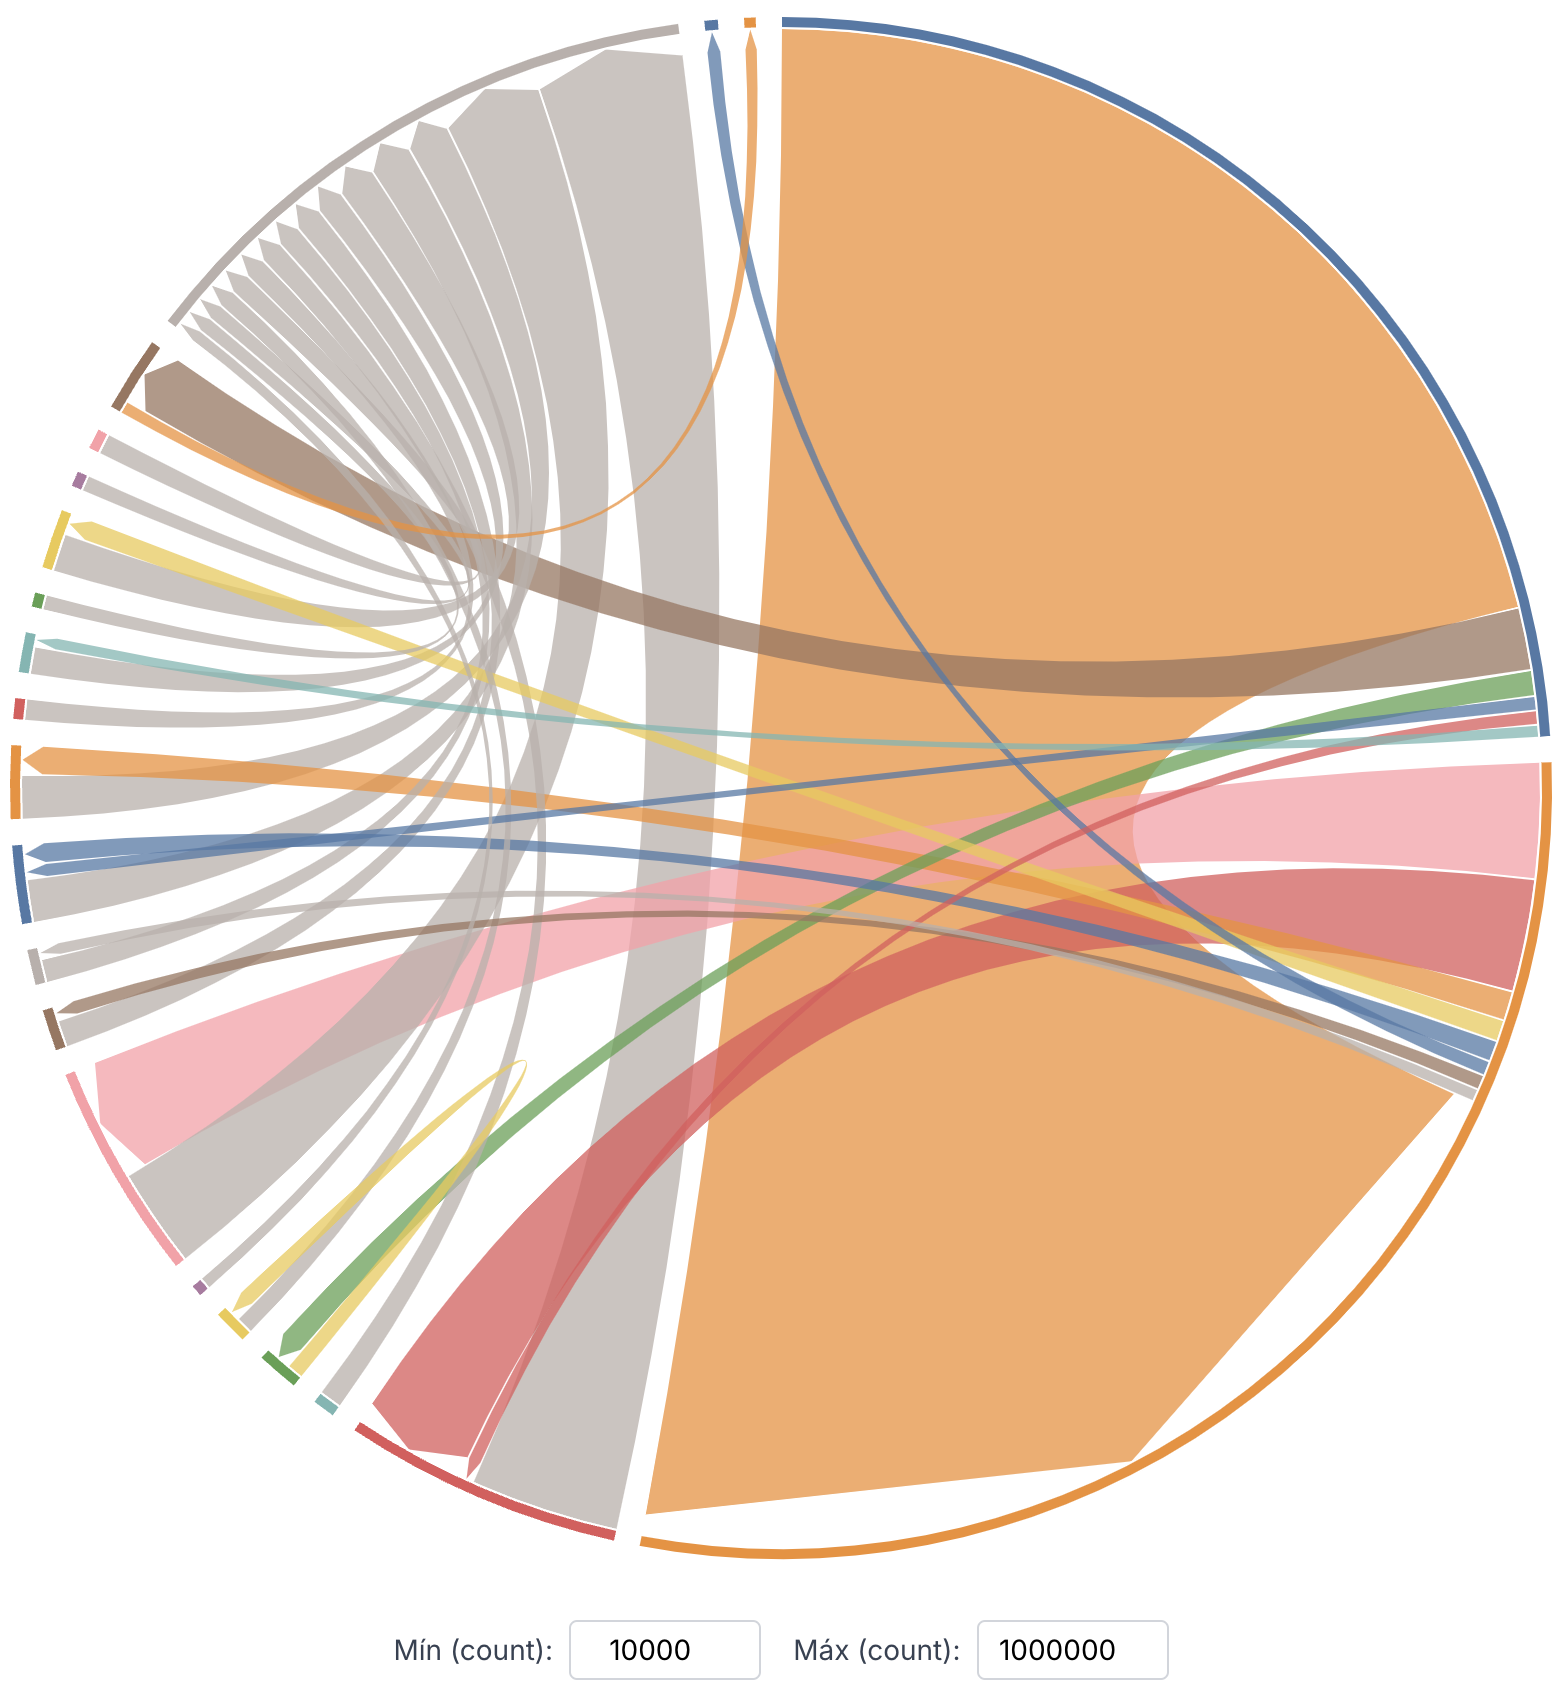
\includegraphics[width=0.88\textwidth]{imagenes/chart-flows.png}}
  \caption{Flujos hospitalarios}
  \label{fig:chart-flows}
\end{figure}


